\section{真實度模型實作}
本研究使用OOP的觀念與特性在Apache Spark上面實做真實度模型,在前面有提到對於資料的真實度評價可以從很多面向來做探討,換句話說,藉由OOP的設計方式可以讓使用者實作出真實度需要包含哪一些屬性,還有真實度的量化方法、權重加成等方法。\\\par
本研究將使用Python 作為我們設計與實作真實度模型的程式語言。原因是Python 不但是物件導向的程式語言,而且那它也是Apache Spark 所支援的程式語言。再來Python是十分易懂且容易學習的程式語言,這樣使用者在理解本模型的實作架構的時候,困難度將大大降低。\\\par
前面XML文件真實度的理論模型的描述方式是由上往下(Top-Down)的描述本研究模型的架構,而這樣描述模型的架構,在轉換成程式實作的時候,會無法使用程式語言描述清楚 ,所以在實作的時候必須採用堆疊式的方法來建構模型,也就是所謂的Bottom-Up的設計方法,本研究在設計API的時侯先將所有屬性設定完成,接著在維度陣列當中添加設計好的屬性,接著在模型陣列當中添加分類好的維度,依這樣的步驟,由下而上的把模型堆疊上去,這樣的模型是有彈性的,因為在要決定屬性隸屬於哪一個維度的時候,如果有別的模型要使用相同的屬性,那只需要把那一個屬性的物件加入到別的模型的維度陣列當中即可,這樣就可以達到相同的屬性量化方式,但是應用到不同模型維度當中,兼具了物件導向當中的彈性設計以及程式碼的重用性。
\subsection{模型實作}
真實度模型的建立,其中最重要的就是彈性以及程式的重用性,也就是用物件導向程式設計的特性來達到程式碼的重用,這在於模型是使用者決定他所認為的兩個文件真實度所具備的屬性,也就是說每個人所認為的真實度不同,在實作上就會有所不同,本研究設計真實度模型的抽象類別,首先對於XML文件真實度而言,設計一個真實度模型(Veracity Model),模型當中會具有多個維度(Dimension $D_i,  i=1\ to\ n$),在每一個維度之下會有多個屬性(Attribute $A_{i, j}, j=1\ to\ n$)來描述此維度,並且每一個維度需要有一個量化方法,對應到物件導向上可以將模型視為一個抽象類別,維度視為一個抽象類別,屬性視為一個抽象類別,所以程式上設計了 Model、Dimension、Attribute三個主要的抽象類別讓使用者去繼承並實作。\\\par
如前面提到因為一個XML文件的真實度是可以有很多面向,換言之就是可以從很多維度去探討,維度裡面會有很多屬性,這一些屬性都會有一個對於XML真實度的量化方式。\\\par
API的最上層是Model,Model底下會有真實度模型的各項元件。而Python本身沒有支援抽象類別的設計,所以要使用Python設計抽象類別就必須載入一個叫做abc的模組,並且在想要抽象的方法前面加入前綴,才能實現抽象類別的設計。整體抽象類別的設計如圖\ref{model}所示,在Model 當中 ,第7行設有dimension的list,用於建立此模型的維度,使用者必須將設計好的1到n個維度傳入這個list當中儲存,利用物件導向的特性,當Dimension的物件與Model的物件產生後,可以將多個Dimension 物件也就是多個維度使用第11行set\_dimension()的方法儲存到 dimension 這個list當中,接著在第15行設計get\_dimension()的方法來取得這個模型下的維度list。而最後需要計算模型的整體分數Veracity Value,所以在第19行設計有 veracity\_value()的方法,用以計算模型的整體分數。

\begin{figure}[H]
\centering
\graphicspath{{/Users/FUDA/Documents/masterThesis/image/}}
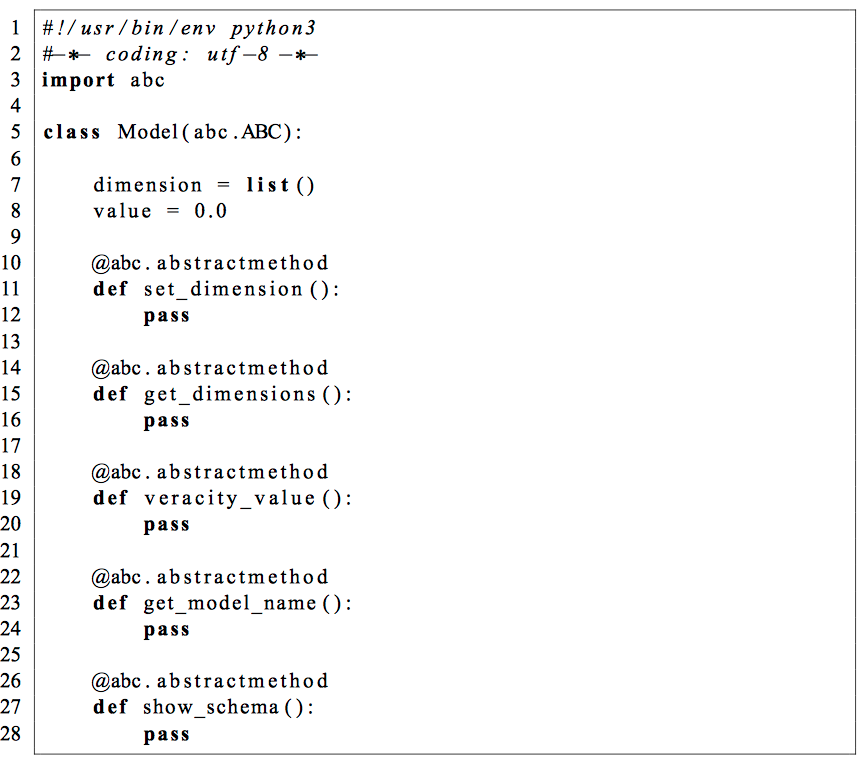
\includegraphics[scale=0.4]{model.png}
\caption{Model 抽象類別設計}
\label{model}
\end{figure}

在模型之下會有多個維度,需建立維度的類別來描述維度的架構,維度抽象類別的設計如圖\ref{dimension}所示,使用第11行set\_attributes()將建立好的屬性物件傳入attributes的 list 當中存起來,這樣就可以用物件導向的的概念去存取到下面屬性的物件的方法。另外實作上要求使用者在繼承維度的時候設定維度名稱,並且可以用第15行的get\_dimension\_name()取得維度名稱。接著需要實作第19行get\_attributes()的方法來取得先前傳入的屬性,在維度當中也會有該維度的計分,所以在第23行dimension\_degree()會設計有維度的計分方法讓使用者實作。

\begin{figure}[H]
\centering
\graphicspath{{/Users/FUDA/Documents/masterThesis/image/}}
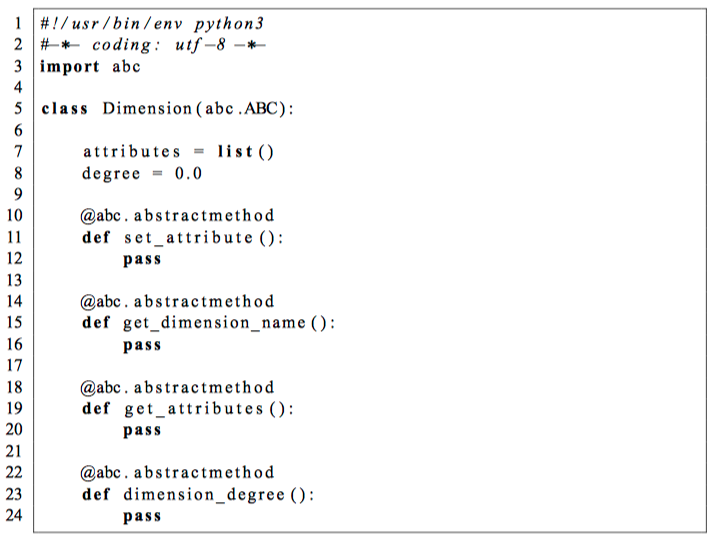
\includegraphics[scale=0.4]{dimension.png}
\caption{Dimension 抽象類別設計}
\label{dimension}
\end{figure}

而在屬性抽象類別當中,設計有兩個方法,分別是get\_attribute\_name()以及quantification(),抽象類別設計如圖\ref{attribute}所示,使用者需繼承這一個類別來實作屬性的量化方式,在get\_attribute\_name()中本實作直接設計這個方法將回傳類別名稱,也就是要求開發者在繼承並且實作的時候,類別名可以直接取成相關的屬性名稱,這樣的設計方式也是為了在存取屬性的時候方便識別。\\\par
\newpage
\begin{figure}[H]
\centering
\graphicspath{{/Users/FUDA/Documents/masterThesis/image/}}
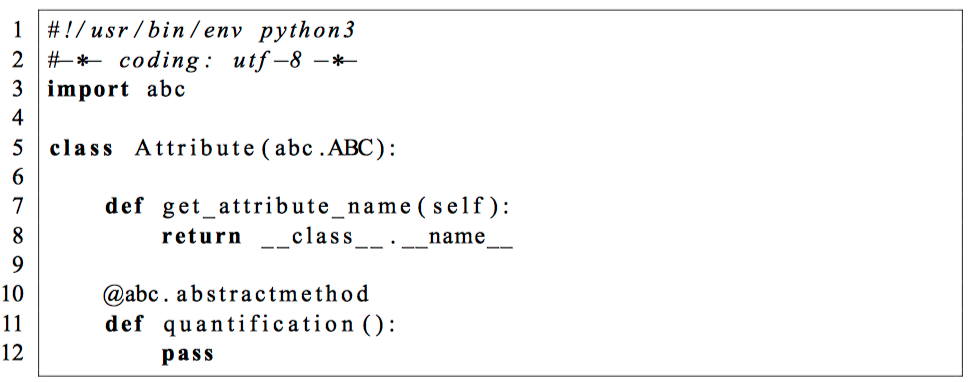
\includegraphics[scale=0.5]{attribute.png}
\caption{Attribute 抽象類別設計}
\label{attribute}
\end{figure}
以上Model、Dimension、Attribute三大類別構成了真實度模型的基礎架構,模型的建立由使用者繼承維這三大類別,使用者須先實作完屬性的量化方式接著產生屬性物件並添加至維度之內,接者再將維度物件添加至模型當中,並且在實作每一個類別的時候,須將抽象類別當中的量化方法實作完畢,接著在模型中計算總體量化的分數。\\\par